\documentclass[tikz,border=14pt]{standalone}
\usepackage{amsmath,amssymb}
\usetikzlibrary{arrows.meta}
\definecolor{ink}{HTML}{E4EDF8}
\definecolor{muted}{HTML}{596B80}
\definecolor{blue}{HTML}{9FC2FF}
\definecolor{teal}{HTML}{63D3BB}
\definecolor{gold}{HTML}{E7C274}
\definecolor{panel}{HTML}{111923}
\pagecolor{panel}
\color{ink}
\begin{document}
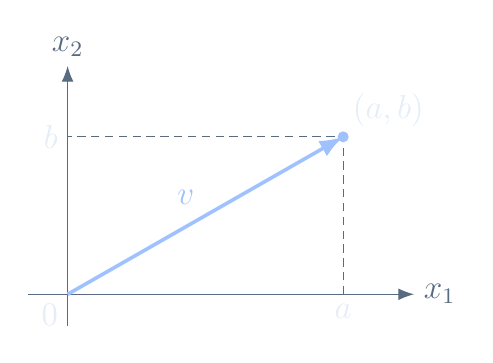
\begin{tikzpicture}[font=\large,text=ink,vec/.style={-{Latex[length=3mm]},line width=1.3pt},axis/.style={muted,-{Latex[length=2mm]},thin}]
\draw[axis] (-.5,0)--(4.4,0) node[right] {$x_1$};
\draw[axis] (0,-.4)--(0,2.9) node[above] {$x_2$};
\node[below left] at (0,0) {$0$};
\draw[densely dashed,muted] (3.5,0)--(3.5,2)--(0,2);
\node[below] at (3.5,0) {$a$};\node[left] at (0,2) {$b$};
\draw[vec,blue] (0,0)--(3.5,2) node[midway,above left] {$v$};
\fill[blue] (3.5,2) circle (2pt) node[above right,text=ink] {$(a,b)$};
\end{tikzpicture}
\end{document}
